\section{Computational experiment}
The goal of this experiment is to select important features and set up baseline patterns for the resulting model. \\
As a basic dataset we use PDBCNN database\cite{database}. For the analysing purposes we retrieve the following information from each experiment - size of the first protein and size of the second protein. Therefore in the basic set we have 647 objects each represented by 2 real features and an affinity target. \\
We split the set into train and validation uniformly from Bernoulli distribution with probability equal to $0.7$. 
Using cross-validation with 3 splits we fit a \textbf{CatBoostRegressor} model on train data.

\begin{center}
\caption{Base CatBoost model performance}
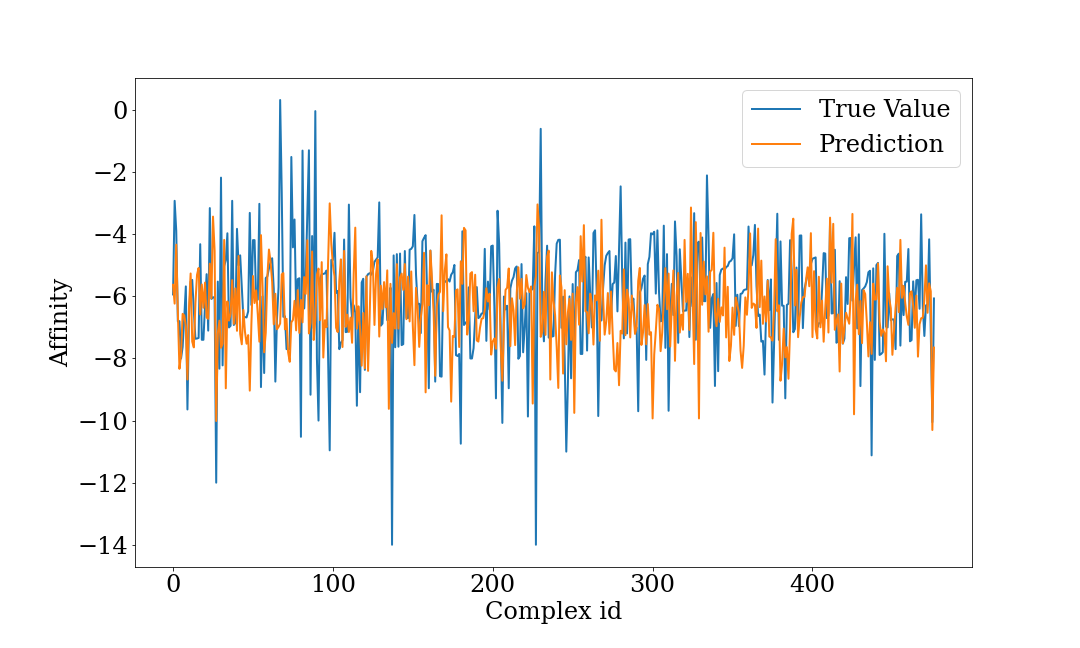
\includegraphics[width=0.8\textwidth]{contents/pred.png}
\end{center}

\begin{center}
\caption{Base CatBoost model errors}
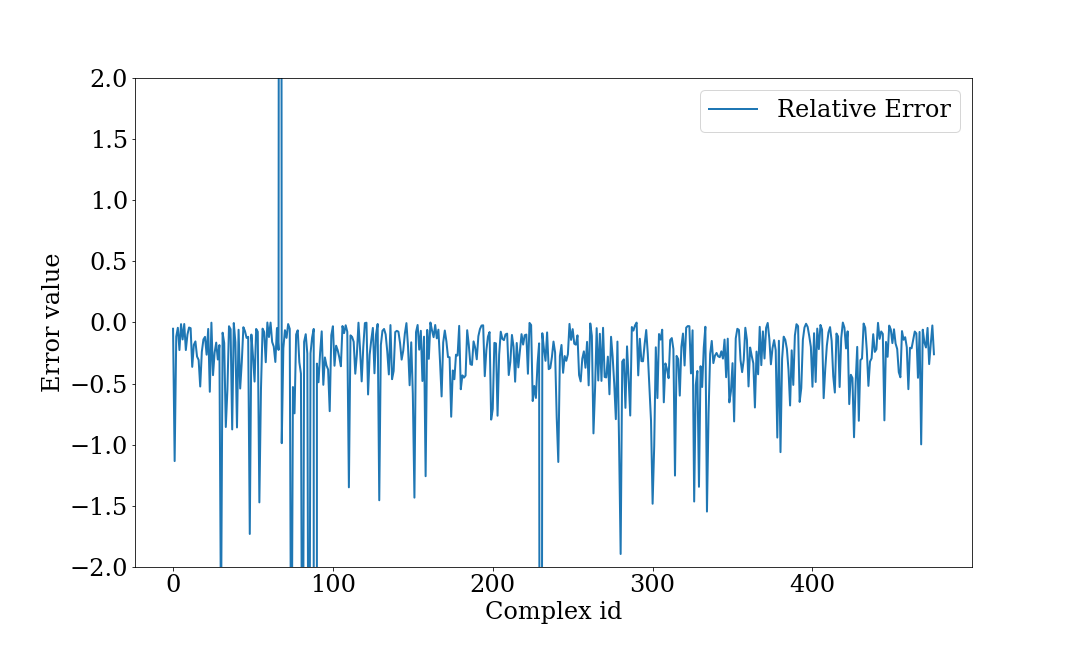
\includegraphics[width=0.8\textwidth]{contents/error.png}
\end{center}

\href{https://catboost.ai/docs/concepts/python-quickstart}{CatBoost} model with default parameters is our base model with MSE of $4.8$. On the figures above one can find a relative error on the test data set and a prediction itself. 
We plan to benchmark our models against existing state-of-the art solutions and this one. Our current suggestions are Graph Neural Network and 3D-CNN.